% Fig 3.7 — Hybrid fusion: CC and RRF side-by-side
\documentclass[border=4pt]{standalone}
\usepackage{amsmath}
\usepackage{tikz}
% Shared TikZ style for thesis figures.
% Each fig_*.tex \input{} this file after \usepackage{tikz}.
% Defines a muted, examiner-friendly color palette and semantic box styles.

\usepackage{xcolor}
\usepackage{fontawesome5}
\usetikzlibrary{positioning, arrows.meta, shapes.geometric, calc, fit, backgrounds}

% ─── Palette ───────────────────────────────────────────────────────────
% Each role has a stroke color (dark) and a fill color (very light).
% Designed to be grayscale-safe — lightness differs enough that B&W printing
% still preserves the distinction.

\definecolor{thQueryS}{HTML}{4A6FA5}    \definecolor{thQueryF}{HTML}{E8EEF6}   % query / input
\definecolor{thLLMS}{HTML}{6D4A8F}      \definecolor{thLLMF}{HTML}{ECE5F2}     % LLM / generation
\definecolor{thRetS}{HTML}{3D7A4F}      \definecolor{thRetF}{HTML}{E4EFE7}     % retriever
\definecolor{thDataS}{HTML}{6A6A6A}     \definecolor{thDataF}{HTML}{F1F1F1}    % corpus / data
\definecolor{thFusionS}{HTML}{A05A30}   \definecolor{thFusionF}{HTML}{F4E8DF}  % fusion
\definecolor{thOutS}{HTML}{1F6F8A}      \definecolor{thOutF}{HTML}{DEEAEF}     % output / final
\definecolor{thHiS}{HTML}{0D4D63}       \definecolor{thHiF}{HTML}{C8D9DF}      % highlighted (our contribution)
\definecolor{thMuted}{HTML}{5C5C5C}

% ─── Box styles ────────────────────────────────────────────────────────
% Usage in tikzpicture options:  query/.style={thQuery}, llm/.style={thLLM}, ...
% Or directly on nodes:          \node[thLLM] (m) {...};
\tikzset{
  thBase/.style={rectangle, draw, rounded corners=2pt,
                 minimum width=28mm, minimum height=10mm,
                 align=center, font=\small, line width=0.6pt,
                 inner sep=4pt},
  thQuery/.style={thBase, draw=thQueryS, fill=thQueryF},
  thLLM/.style={thBase, draw=thLLMS, fill=thLLMF},
  thRet/.style={thBase, draw=thRetS, fill=thRetF},
  thData/.style={cylinder, shape border rotate=90, aspect=0.3, draw=thDataS, fill=thDataF,
                 minimum width=24mm, minimum height=12mm, align=center, font=\small, line width=0.6pt},
  thFusion/.style={thBase, draw=thFusionS, fill=thFusionF},
  thOut/.style={thBase, draw=thOutS, fill=thOutF},
  thHi/.style={thBase, draw=thHiS, fill=thHiF, line width=1pt},
  thArrow/.style={-{Stealth[length=2.5mm]}, line width=0.7pt, draw=thMuted},
  thLabel/.style={font=\footnotesize\itshape, color=thMuted},
  thStage/.style={font=\bfseries\footnotesize, color=thMuted},
}

% ─── Icon helpers ──────────────────────────────────────────────────────
% Tiny FontAwesome icons that can sit inside a node prefix.
% Usage:  \node[thQuery] {\thIconQuery~User query};
\newcommand{\thIconQuery}{\textcolor{thQueryS}{\faSearch}}
\newcommand{\thIconUser}{\textcolor{thQueryS}{\faUser}}
\newcommand{\thIconLLM}{\textcolor{thLLMS}{\faBrain}}
\newcommand{\thIconRet}{\textcolor{thRetS}{\faNetworkWired}}
\newcommand{\thIconCorpus}{\textcolor{thDataS}{\faDatabase}}
\newcommand{\thIconFusion}{\textcolor{thFusionS}{\faCodeBranch}}
\newcommand{\thIconOut}{\textcolor{thOutS}{\faFile}}
\newcommand{\thIconEval}{\textcolor{thOutS}{\faChartBar}}
\newcommand{\thIconStar}{\textcolor{thHiS}{\faStar}}
\newcommand{\thIconCog}{\textcolor{thMuted}{\faCog}}


\begin{document}
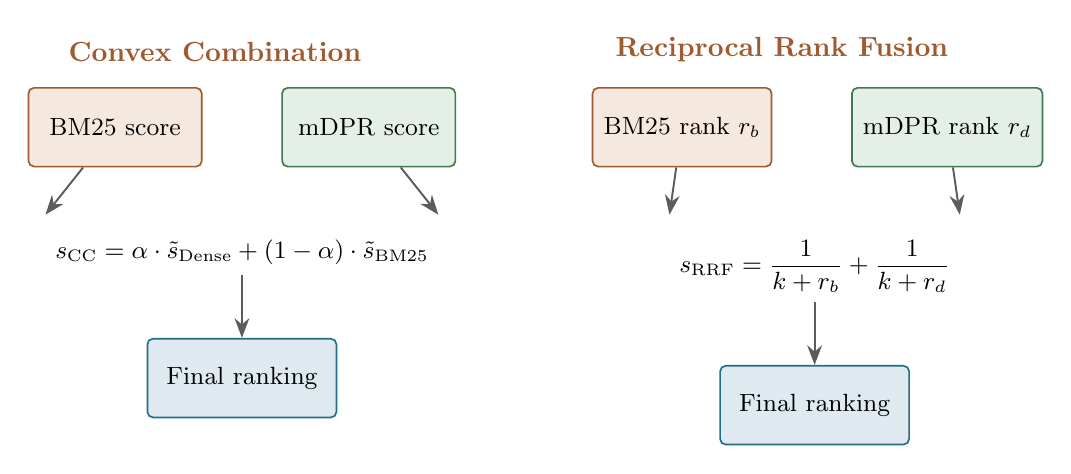
\begin{tikzpicture}[node distance=8mm and 10mm]
  % --- CC half ---
  \node[thFusion, minimum width=22mm] (bm1) {BM25 score};
  \node[thRet, minimum width=22mm, right=of bm1] (dn1) {mDPR score};
  \node[font=\small, below=8mm of $(bm1.south)!0.5!(dn1.south)$] (cc) {%
      $s_{\text{CC}} = \alpha \cdot \tilde{s}_{\text{Dense}} + (1-\alpha)\cdot\tilde{s}_{\text{BM25}}$};
  \node[thOut, minimum width=24mm, below=of cc] (rcc) {Final ranking};

  \draw[thArrow] (bm1) -- ($(cc.north west)+(0,2mm)$);
  \draw[thArrow] (dn1) -- ($(cc.north east)+(0,2mm)$);
  \draw[thArrow] (cc) -- (rcc);
  \node[font=\bfseries, color=thFusionS, above=2mm of bm1, xshift=12mm] {\thIconFusion~Convex Combination};

  % --- RRF half ---
  \begin{scope}[xshift=72mm]
    \node[thFusion, minimum width=22mm] (bm2) {BM25 rank $r_b$};
    \node[thRet, minimum width=22mm, right=of bm2] (dn2) {mDPR rank $r_d$};
    \node[font=\small, below=8mm of $(bm2.south)!0.5!(dn2.south)$] (rrf) {%
        $s_{\text{RRF}} = \dfrac{1}{k + r_b} + \dfrac{1}{k + r_d}$};
    \node[thOut, minimum width=24mm, below=of rrf] (rrr) {Final ranking};

    \draw[thArrow] (bm2) -- ($(rrf.north west)+(0,2mm)$);
    \draw[thArrow] (dn2) -- ($(rrf.north east)+(0,2mm)$);
    \draw[thArrow] (rrf) -- (rrr);
    \node[font=\bfseries, color=thFusionS, above=2mm of bm2, xshift=12mm] {\thIconFusion~Reciprocal Rank Fusion};
  \end{scope}
\end{tikzpicture}
\end{document}
